\documentclass[a4paper]{article}

%% Language and font encodings
\usepackage[czech]{babel}
\usepackage[utf8]{inputenc}
\usepackage[T1]{fontenc}

%% Table on two pages
\usepackage{booktabs}
\usepackage{tabularx}
\usepackage{ltablex} 
\usepackage{longtable}


\usepackage{xcolor}
\usepackage{listings}

\lstset{language=c,
                keywordstyle=\color{blue},
                stringstyle=\color{red},
                commentstyle=\color{gray},
                morecomment=[l][\color{magenta}]{\#}
}

%% Sets page size and margins
\usepackage[a4paper,top=3cm,bottom=2cm,left=3cm,right=3cm,marginparwidth=1.75cm]{geometry}

%% Useful packages
\usepackage{amsmath}
\usepackage{graphicx}
\usepackage[colorlinks=true, allcolors=blue]{hyperref}

\title{Projekt IMP \\ ARM na FITkit3: sada demo aplikací nad FreeRTOS}
\author{Jaroslav Páral (xparal02)}

\begin{document}
\maketitle

% ---------------------------
% ---------------------------
\section{Úvod}
Cílem projektu bylo nejprve naprogramovat jednoduchý bare-metal projekt (bez operačního systému), který by demonstroval využití základních komponent (tlačítko, LED, piezo) na výukovém kitu FITkit3 (obrázek \ref{fitkit3-foto}). Následně tento projekt upravit tak, aby při obsluze těchto periferií používat operační systém \href{http://www.freertos.org/}{FreeRTOS}. Součástí projektu měla být i dokumentace popisující realizaci zadání.

\subsection{Osobní cíl}
Toto téma jsem si vybral, jelikož jsem v nedávné době dostal k dispozici několik vývojových kitů Freedom od firmy Freescale (dnes již NXP, v budoucnu Qualcomm) za účelem výuky programování mikrokontrolérů v robotickém kroužku na mé bývalé střední škole (SPŠ a VOŠ Brno, Sokolská).  Věděl jsem, že na FITkitu3 je osazen mikrokontrolér od Freescalu a připadalo mi to jako vhodná cesta k seznámení se do hloubky s platformou, kterou Freescale poskytuje. Domluvil jsem si i s zadavatelem projektu na využití Freedom kitů místo požadovaného FITkitu.

\section{Použité prostředky}

Ke splnění projektu byly využity jak hardwarové, tak softwarové prostředky, které bych rád popsal v této části.

\subsection{Hardware}

K řešení projektu jsem plánoval použít vývojové kity \href{http://www.nxp.com/products/software-and-tools/hardware-development-tools/freedom-development-boards/freedom-development-platform-for-kinetis-kl3x-and-kl4x-mcus:FRDM-KL46Z?tid=vanFRDM-KL46Z}{FRDM-KL46Z} (obrázek \ref{frdm-kl46z-pins-description}) a \href{http://www.nxp.com/products/software-and-tools/hardware-development-tools/freedom-development-boards/freedom-development-platform-for-kinetis-k64-k63-and-k24-mcus:FRDM-K64F?tid=vanFRDM-K64F}{FRDM-K64F} (obrázek \ref{frdm-k64f-pins-description}), které mám k dispozici ve větším počtu. Bohužel se mi při řešení projektu vyskytli potíže s oběma kity (u FRDM-K64F se mi nepodařilo zprovozni programování přes vývojového prostředí a na FRDM-KL46Z mi nechtěl fungovat FreeRTOS) a proto jsem nakonec projekt vypracoval na FITkit3. 


\subsection{Programování}
K programování jsem využil vývojové IDE\footnote{Integrated development environment} Kinetis Design Studio (KDS), které poskytuje Freescale zdarma a jedná se prakticky o nadstavbu do Eclipse. Součásti toho IDE je podpůrný nástroj s názvem Processor Expert, který by měl umožnit rychlé a snadné nastavení jednotlivých komponent v mikrokontroléru a následné předvedení například produktu u zákazníka. S tímto cílem byl tento nástroj vyvíjen (není určen pro programování koncových produktů) a možná to je jeho největší problém. Na závěr musím ještě zmínit SDK\footnote{Software development kit}, která si lze od Freescalu stáhnout a využívat je pro vývoj. SDK je k dispozici v několika vývojových verzích (aktuální verze jsou Kinetis SDK v1.3 a~v2.0), s tím že jednotlivé verze mezi sebou nemusí být kompatibilní (v2.0 je úplně odlišné od~v1.3). SDK jsou vytvořena tak, aby Vám umožňovali využít plný výkon zařízení a nenarazili na omezení, způsobená použitím SDK, tím vám urychlili vývoj (v porovnání s čistým zápisem do registru). Na druhou stranu nenabízí takový komfort používání (např. jednoduchá konfigurace komponent) jako Processor Expert.
   
\section{Způsob realizace}

%\subsection{Počáteční varianta}
Jelikož jsem věděl, že Processor Expert (dále už jen PEx) velmi ulehčuje nastavování a zprovozňování jednotlivých komponent, chtěl jsem vše realizovat přes něj.

Začal jsem tedy experimentovat v rámci bare-metal projektu, kde jsem si chtěl vše odzkoušet a následně jen převést pod FreeRTOS. Opravdu mě zajímali možnosti vývoje v KDS a chtěl jsem jej i srovnat s platformou \href{www.mbed.org}{Mbed}. Hned po tom, co jsem se rozhodl používat PEx s SDK, nastali první problémy. Bohužel mnoho součástek z SDK a PEx má mezi sebou kolize a závislosti, proto lze využívat jen omezenou sadu komponent z PEx. Dost často se pak stává, že potřebná komponenta není k danému procesoru (v konfiguraci SDK a PEx) k dispozici. Což velmi komplikuje vývoj. 

Po zjištění těchto problémů jsem se pokus nastudovat si o~PEx a~SDK, co možná nejvíce informací. Bohužel mi připadá, že dokumentace PEx je víc než chabá a~podklady k SDK jsou sice obsáhle, ale stále nedostačující (např. příklady by mohli být více rozepsané).

Největší zádrhel ovšem nastal, když jsem chtěl aktivovat v projektu systém FreeRTOS. Ačkoliv to na počátku vypadalo, že je to otázka maximálně několika minut, opak byl pravdou. 

Přidání FreeRTOS proběhlo vždy zdánlivě v pořádků, ale při následném programování jsem zjistil, že mnou definovaný Task se provede vždy jen jednou a nikdy více. Na tomto problémů jsem strávil minimálně jeden den a ačkoliv jsem prostudoval několik desítek tutoriálů, návodů a~doporučení, řešení jsem nenašel. Už jsem začínal být zoufalý, ale naštěstí se ke mě dostala rada, že mám využít SDK v2.0 (do té doby jsem používal SDK v1.3). 

Z počátku se mi tato varianta nezamlouvala, jelikož to pro mě znamenalo nemožnost využití PEx komponent. Nakonec jsem ale SDK v2.0 použil a naprogramoval FreeRTOS pomocí něj. Musel jsem nastudovat některé části více do hloubky a některé části neimplementovat, ale výsledkem je funkční zařízení s operačním systém. 

\subsection{Finální implementace}

V předešlém textu byly popsáný moje plány a problémy, s kterými jsem se setkal. Nyní bych rád rozebral finální řešení.

Po zmíněných problém jsem se rozhodl projekt implementovat na výukovém kitu FITkit3. Mohl jsem, ale použít i FRDM-KL46Z, u které byl původně problém zprovoznit FreeRTOS, ale po přechodu na SDK v2.0 by již tento problém nemusel nastat.

Rozhodl jsem se pro ukázkovou implementaci obsluhy dvou periferií (LED\footnote{Light-Emitting Diode} a tlačítka). 

V rámci bare-metal projektu jsem využil komponenty z PEx a SDK v1.3, které mi usnadnili nastavení. Pomocí PEx jsem si nastavil, na kterých pinech jsou jednotlivé periferie umístěny a v jakém módu mají pracovat (input/output, pull-up/pull-down,...). Také jsem si nastavil přerušení při sestupné hraně na pinech, kde byli připojena tlačítka. V \verb|main|funkci běžela nekonečná smyčka, která dle nastavené periody blikala s jednou LED a v rámci přerušení jsem zpracovával stisknutí tlačítek, přenastavování periody blikání LED v \verb|main| funkci a rozsvěcování dalších LED v závislosti na zmáčknutém tlačítku. Konkrétní implementaci si lze prohlédnout v projektu \href{https://github.com/JarekParal/IMP-project/tree/master/projects/KDS_FITkit3_bare-metal_KSDK1.3_PEx}{KDS\_FITkit3\_bare-metal\_KSDK1.3\_PEx}. 

\begin{lstlisting}[language=c]
// KDS_FITkit3_bare-metal_KSDK1.3_PEx - main.c
int main(void)
{
  // init
  PE_low_level_init();
  GPIO_DRV_WritePinOutput(MCU_LED0, 0);
  GPIO_DRV_WritePinOutput(MCU_LED1, 1);
  GPIO_DRV_WritePinOutput(MCU_LED2, 1);
  GPIO_DRV_WritePinOutput(MCU_LED3, 1); 
 
  for(;;) {
    GPIO_DRV_TogglePinOutput(MCU_LED0);
    WAIT1_Waitms(LedPeriod);
  }
  // ... 
}
\end{lstlisting}

\newpage

\begin{lstlisting}[language=c]
// Events.c
void PORTE_IRQHandler(void)
{
  if(GPIO_DRV_IsPinIntPending(MCU_BUTTON0))
    if(position > 1)
      position--;
  if(GPIO_DRV_IsPinIntPending(MCU_BUTTON2))
    if(position < 3)
      position++;

  if(GPIO_DRV_IsPinIntPending(MCU_BUTTON1))
    LedPeriod += LedPeriodAddConst;
  if(GPIO_DRV_IsPinIntPending(MCU_BUTTON3))
    if(LedPeriod != 100)
      LedPeriod -= LedPeriodAddConst;

  GPIO_DRV_WritePinOutput(MCU_LED1, 1);
  GPIO_DRV_WritePinOutput(MCU_LED2, 1);
  GPIO_DRV_WritePinOutput(MCU_LED3, 1);

  switch(position)
  {
    case 1:
      GPIO_DRV_WritePinOutput(MCU_LED1, 0);
      break;
    case 2:
      GPIO_DRV_WritePinOutput(MCU_LED2, 0);
      break;
    case 3:
      GPIO_DRV_WritePinOutput(MCU_LED3, 0);
      break;
  }

  /* Clear interrupt flag.*/
  PORT_HAL_ClearPortIntFlag(PORTE_BASE_PTR);
  /* Write your code here ... */
}  
\end{lstlisting}

Varianta projektu s FreeRTOS se lišila tím, že nevyužívala PEx a místo SDK v1.3 bylo použito SDK v2.0. Pro inicializaci komponent MCU jsem použil makra, která byla částečně přejata z PEx a přistupovali přímo k registrům. V  \verb|main| funkci proběhla inicializace všech komponent a dvou \verb|tasku|. První task \verb|led_task| zajišťoval blikání LED podle dané periody. Druhý task \verb|btn_task| zpracovával stisky tlačítek a následně upravoval periodu blikání LED v \verb|led_task| a nebo přepínal stav tří signalizačních LED (uživatel mohl určovat, která ze tří LED má svítit a pomocí dvou tlačítek posouval svítící LED doprava/doleva). Implementaci lze najít v projektu \href{https://github.com/JarekParal/IMP-project/tree/master/projects/FDS_FITkit3_FreeRTOS_KSDK2.0}{FDS\_FITkit3\_FreeRTOS\_KSDK2.0}.


\begin{lstlisting}[language=c]
int main(void) {
  // Init boadr ...
  /* Create RTOS task */
  xTaskCreate(led_task, "led_task", configMINIMAL_STACK_SIZE, NULL, 
    led_task_PRIORITY, NULL);
  xTaskCreate(btn_task, "btn_task", configMINIMAL_STACK_SIZE, NULL, 
    btn_task_PRIORITY, NULL);
  vTaskStartScheduler();

  for(;;) { /* Infinite loop to avoid leaving the main function */
    __asm("NOP"); /* something to use as a breakpoint stop while looping */
  }
} 
\end{lstlisting}

\begin{lstlisting}[language=c]
static void btn_task(void *pvParameters) 
{
  for (;;) {
    if(GPIO_ReadPinInput(MCU_BUTTON1_GPIO, MCU_BUTTON1_GPIO_PIN) == 0)
      if(led_period > 100)
        led_period -= dif_led_period;
    if(GPIO_ReadPinInput(MCU_BUTTON3_GPIO, MCU_BUTTON3_GPIO_PIN) == 0)
      if(led_period < 2000)
        led_period += dif_led_period;
  
    if(GPIO_ReadPinInput(MCU_BUTTON0_GPIO, MCU_BUTTON0_GPIO_PIN) == 0 
      && BTN0_LAST == 1) 
    {
      BTN0_LAST = 0;
      if(position > 1)
        position--;
    } else {
      BTN0_LAST = GPIO_ReadPinInput(MCU_BUTTON0_GPIO, MCU_BUTTON0_GPIO_PIN);
    }
    if(GPIO_ReadPinInput(MCU_BUTTON2_GPIO, MCU_BUTTON2_GPIO_PIN) == 0 
      && BTN2_LAST == 1) 
    {
      BTN2_LAST = 0;
      if(position < 3)
        position++;
    } else {
      BTN2_LAST = GPIO_ReadPinInput(MCU_BUTTON2_GPIO, MCU_BUTTON2_GPIO_PIN);
    }
  
    MCU_LED1_OFF();
    MCU_LED2_OFF();
    MCU_LED3_OFF();
    switch(position)
    {
      case 1:
        MCU_LED1_ON();
        break;
      case 2:
        MCU_LED2_ON();
        break;
      case 3:
        MCU_LED3_ON();
        break;
    }
    vTaskDelay(50/portTICK_RATE_MS); // control every 50 ms
  }
}

static void led_task(void *pvParameters) 
{
  for (;;) {
    MCU_LED0_TOGGLE();
  
    vTaskDelay(led_period/portTICK_RATE_MS);
  }
}
\end{lstlisting}

 

\section{Porovnáni s platformou Mbed}

Platforma Mbed se snaží nabídnout podobně jednoduchý přístup pro programování mikrokontrolérů jako platforma \href{https://www.arduino.cc/}{Arduino}. Ovšem Mbed je postaven primárně na ARMech a snaží se splňovat i určité průmyslové standardy. V porovnání s KDS nabízí výrazně jednoduší a srozumitelnější vývojové prostředí se základními možnostmi. Naopak oproti KDS (a případně PEx) oproti Mbedu nabízí rozsáhlejší knihovny i podklady a umožňuje jít více k hardwaru.

\begin{lstlisting}[language=c]
// mbed-rtos
DigitalOut led1(LED1);
DigitalOut led2(LED2);

void led2_thread(void const *argument) {
    while (true) {
        led2 = !led2;
        Thread::wait(500);
        print_char();
    }
}

int main() {
    Thread thread(led2_thread, NULL, osPriorityNormal, STACK_SIZE);

    while (true) {
        led1 = !led1;
        Thread::wait(500);
    }
}

\end{lstlisting}

\newpage

\section{Závěr}
Výsledkem mého projektu jsou dvě aplikace (bare-metal a s FreeRTOS), které řídí 4 LED osazené na FITkitu a zpracovávají vstupy z tlačítek (tím lze určit stav LED). Bare-metal varianta je asi o trochu jednoduší, což je způsobeno hlavně použitím PEx. Každá varianta má své výhody. V bate-metal aplikaci je použit interrupt pro snímání zmáčknutí tlačítka. Naopak ve FreeRTOSu jsem využil jedno vlákno pro snímání tlačítek a druhé vlákno pro ovládání periody blikání LED. V RTOS variantě by se dali vlákna využít lépe avšak po problémech se zprovozněním FreeRTOS a při omezením množství periferií na FITkity jsem další varianty nerealizoval.

Můžete se podívat na video předvádějící fungování programu: \url{https://youtu.be/nl1vykVDIRg}

Celý projekt (s kompletními projekty) lze najít na GitHubu. Jsou zde dostupné i projekty, které jsem vypracoval pro FRDM-KL46Z: \url{https://github.com/JarekParal/IMP-project}


\begin{figure}[h]
	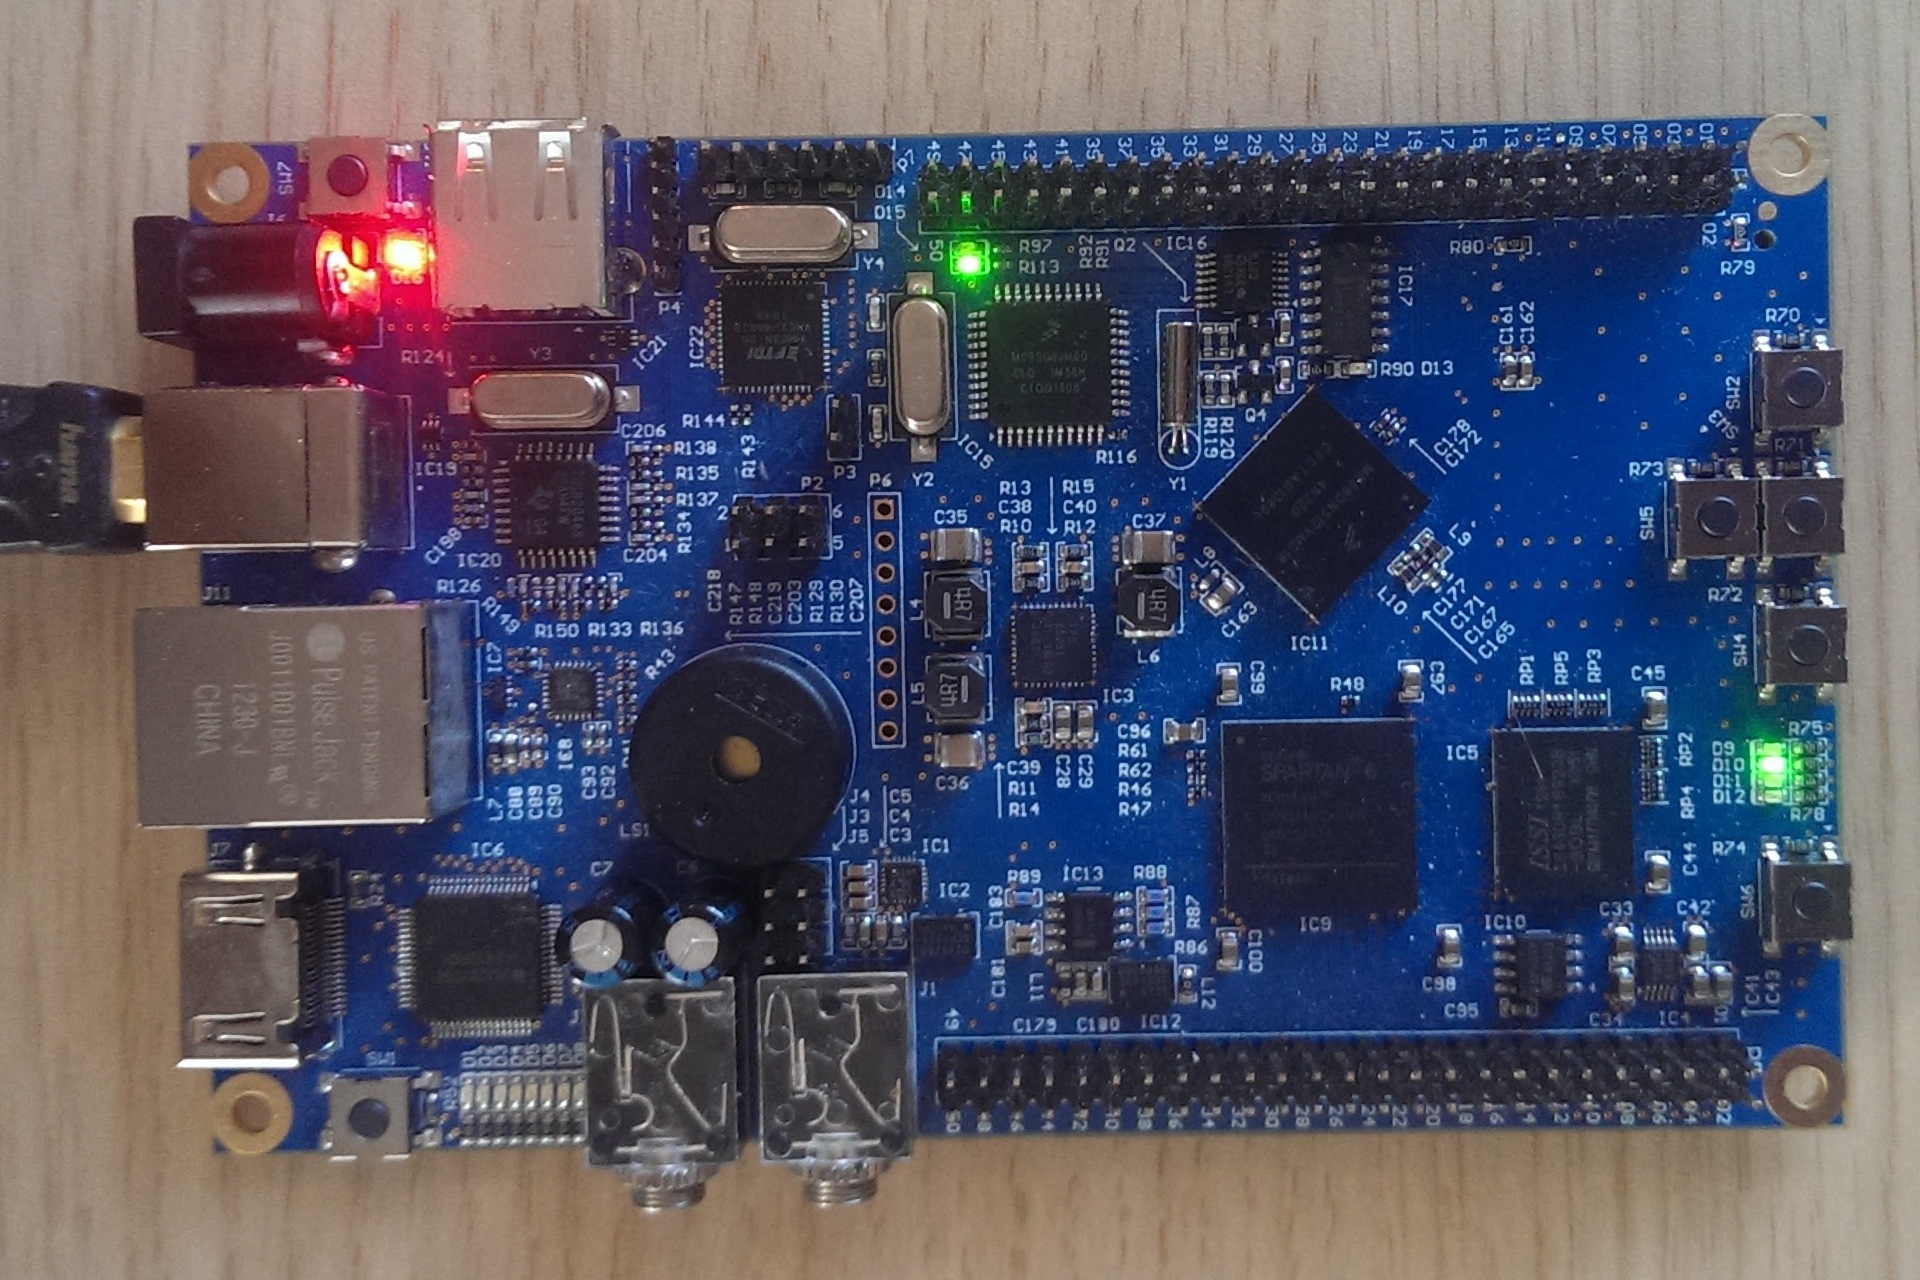
\includegraphics[width=\textwidth]{fitkit3-foto.jpg}
	\caption{Výukový kit FITkit3}
	\label{fitkit3-foto}
\end{figure}


\newpage
\section*{Přílohy}

\begin{figure}[h]
	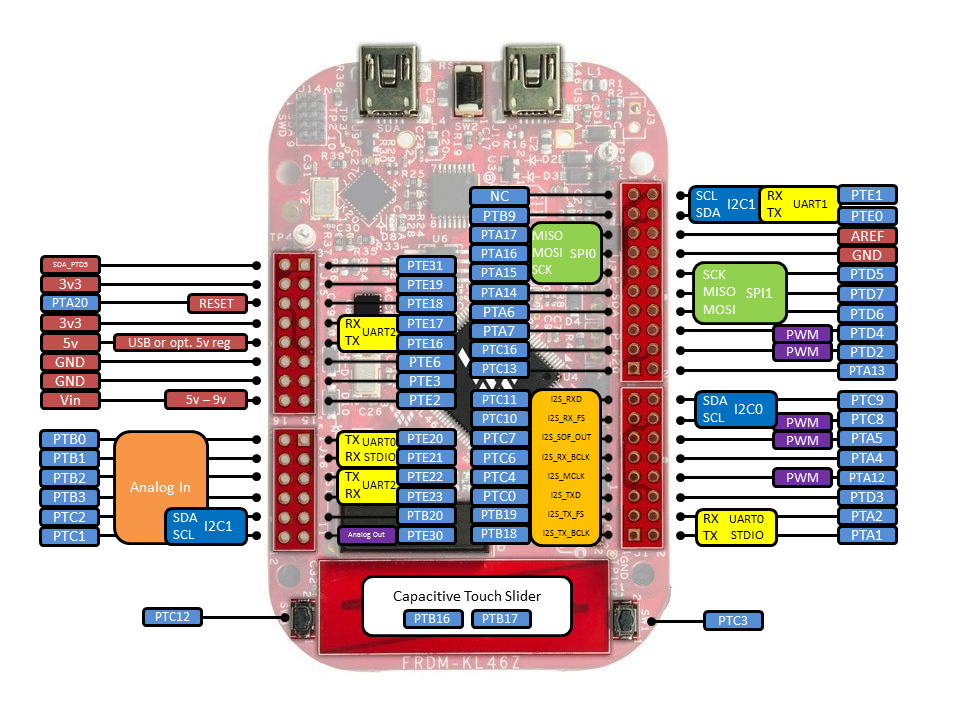
\includegraphics[width=\textwidth]{frdm-kl46z-pins-description.png}
	\caption{Vývojový kit FRDM-KL46Z}
	\label{frdm-kl46z-pins-description}
\end{figure}

\begin{figure}[h]
	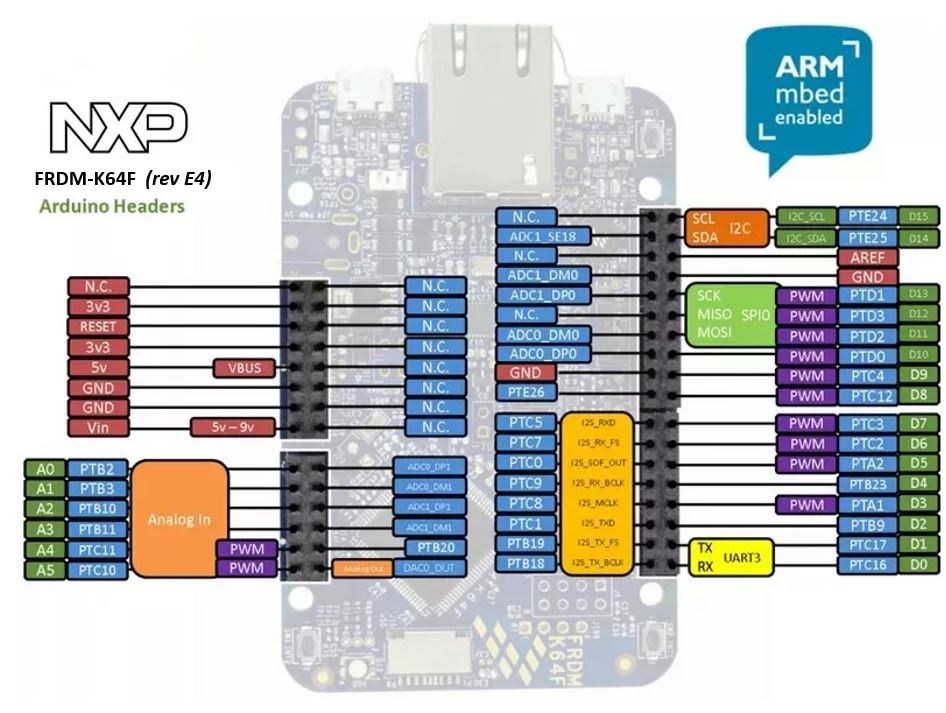
\includegraphics[width=\textwidth]{frdm-k64f-pins-description.jpg}
	\caption{Vývojový kit FRDM-K64F}
	\label{frdm-k64f-pins-description}
\end{figure}

\end{document}